\section{Partiella differentialekvationer}

\paragraph{Dirichletvillkor}
Betrakta en differentialekvation som skall lösas på ett domän $\Omega$. Dirichletvillkor är på formen 
\begin{align*}
	u(x, t) = 0, x\in\bound{\Omega}.
\end{align*}

\paragraph{Neumannvillkor}
Betrakta en differentialekvation som skall lösas på ett domän $\Omega$. Neumannvillkor är på formen
\begin{align*}
	n_{i}\del{i}{u(x, t)} = 0, x\in\bound{\Omega},
\end{align*}
där $n$ är normal på $\bound{\Omega}$.

\paragraph{Robinvillkor}
Betrakta en differentialekvation som skall lösas på ett domän $\Omega$. Robinvillkor är på formen
\begin{align*}
	\alpha(x, t)u(x, t) + \beta(x, t)n_{i}\del{i}{u(x, t)} = 0, x\in\bound{\Omega},
\end{align*}
där $n$ är normal på $\bound{\Omega}$.

\paragraph{Homogena och inhomogena grejer}
En differentialekvation på formen
\begin{align*}
	Lu = f
\end{align*}
kallas för homogen om $f = 0$ och inhomogen annars. Vi definierar homogena och inhomogena randvillkor analogt.

\paragraph{Flerdimensionell variant av Sturm-Liouvilles sats}
Problemet
\begin{align*}
	&\laplace{f} = \lambda f, \\
	&f(x) = 0, x\in\bound{\Omega}
\end{align*}
har oändligt många lösningar $f_{n}$ med distinkta egenvärden $\lambda_{n} > 0$ så att lösningarna bildar en fullständig mängd och är ortogonala med inreprodukten
\begin{align*}
	\inprod{f}{g} = \integ[n]{\Omega}{x}{\cc{f}(x)g(x)}.
\end{align*}

För problemet
\begin{align*}
	&\laplace{f} = \lambda f, \\
	&\alpha(x, t)u(x, t) + \beta(x, t)n_{i}\del{i}{u(x, t)} = 0, x\in\bound{\Omega},
\end{align*}
där $n$ är normal på $\bound{\Omega}$, finns det oändligt många ortogonala lösningar med distinkta egenvärden, där dessa bildar en fullständig mängd.

\paragraph{Spektralsatsen}
Låt $A$ vara en självadjungerad operator med diskret spektrum. Då har $A$ oändligt många egenfunktioner. Dessa är ortogonala och bildar en fullständig mängd.

\paragraph{Lösning av PDE:er for dummies}
\begin{figure}[!ht]
	\centering
	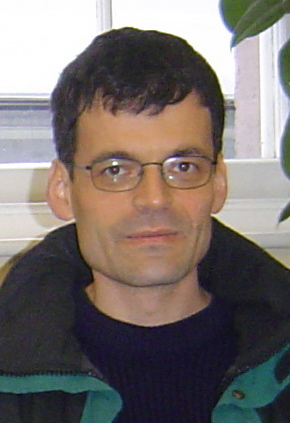
\includegraphics[width = 0.2\textwidth]{./Images/langmann.jpg}
	\caption{Peak fysiker.}
	\label{fig:langmann}
\end{figure}
Fysiker hatar honom. Här kan du läsa hans tre enkla steg för att göra teoretisk fysik komplett vid att lösa partiella differentialekvationer:
\begin{enumerate}
	\item Bestäm lösningar till det homogena problemet.
	\item Välj lösningar som passar till randvillkoren. Sturm-Liouvilles sats garanterar att det finns lösningar. Låt den allmänna lösningen vara en linjärkombination av dessa.
	\item Hitta motsvarande lösningar till variabler som inte har randvillkor.
	\item Skriv upp den allmänna lösningen som en linjärkombination av lösningarna du har fått innan.
	\item Välj koefficienter som passar till initialvillkoren. Det finns även satser som hjälper med detta.
\end{enumerate}

\paragraph{Separationsmetoden}
Separationsmetoden är ett sätt att lösa homogena partiella differentialekvationer på.

Låt $u(x_{1}, \dots, x_{n})$ vara en lösning till $Lu = 0$, där $L$ är en linjär differentialoperator. Separationsmetoden går ut på att göra ansatsen
\begin{align*}
	u = \prod\limits_{i = 1}^{n}X_{i}(x_{i}).
\end{align*}
Denna ansatsen gör förhoppningsvis att differentialekvationen kan skrivas som
\begin{align*}
	\frac{1}{X_{1}}L_{1}X_{1} = \frac{1}{\prod\limits_{i = 1}^{n}X_{i}}L'\prod\limits_{i = 1}^{n}X_{i}.
\end{align*}
Varje sida beror av olika variabler, varför de måste vara lika med en konstant. På detta sättet kan det ursprungliga problemet förhoppningsvis separeras i delproblem som är enkla att lösa.

\paragraph{Lösningsstrategi för inhomogena problem}
Om man har ett problem med inhomogeniteter i differentialekvationen och/eller villkoren, finns det olika strategier för att lösa detta problemet:
\begin{itemize}
	\item dela upp lösningen i en homogen och partikulär lösning. Den partikulära lösningen fås då vid att gissa en lösning.
	\item flytta inhomogeniteten från villkoren till differentialekvationen, för sen att försöka lösa det.
	\item serieutveckla ekvationen och lösningen, vilket ger ett ODE-problem för basfunktionerna.
\end{itemize}
Här specifieras hur metod två fungerar.

För att utdypa kring andra metoden, betrakta ekvationen
\begin{align*}
	Lu            &= 0, \\
	Au(\vb{x}, t) &= f(\vb{x}, t), x\in\bound{\Omega},
\end{align*}
där både $L$ och $A$ är linjära operatorer. Antag att man hittar en funktion $w$ som uppfyller $Aw = f$ på randen, och inför $v = u - w$, där $u$ är en lösning. Denna uppfyller
\begin{align*}
	\del{t}{v} + Lv = \del{t}{u} + Lu - \del{t}{w} - Lw = -\del{t}{w} - Lw,
	Av(\vb{x}, t) = 0, x\in\bound{\Omega}.
\end{align*}

\paragraph{Greenfunktioner}
För att prata om Greenfunktioner, behöver vi först introducera integralkärnor. Om en linjär operator $L$ på ett intervall $I$ uppfyller
\begin{align*}
	Lf(x) = \integ{I}{y}{K(x, y)f(y)},
\end{align*}
säjs $K$ vara integralkärnan till $L$. Detta kan definieras analogt i flera dimensioner.

Betrakta nu differentialekvationen
\begin{align*}
	Lf = g
\end{align*}
i $d$ dimensioner på området $\Omega$ med homogena randvillkor och begynnelsevillkor. Nu har $L$ givetvis ingen integralkärna, då det är en derivationsoperator. Däremot kan $L^{-1}$ tänkas ha det. Antag vidare att $L^{-1}$ har integralkärnan $G$. Då skulle lösningen på problemet ovan vara
\begin{align*}
	f = \integ[d]{\Omega}{y}{G(x, y)g(y)}.
\end{align*}
Vi definierar då $G$ att vara Greenfunktionen till $L$.

Hur kan vi hitta Greenfunktioner till en given operator? Vi använder superpositionsprincipen
\begin{align*}
	Lf_{1} = g_{1}, Lf_{2} = g_{2} \implies L(f_{1} + f_{2}) = g_{1} + g_{2}.
\end{align*}
Detta implicerar att om vi kan dela upp $g$ i hanterbara delar och lösa
\begin{align*}
	Lf_{i} = g_{i},
\end{align*}
kan vi hitta Greenfunktionen. Vi väljer uppdelningen
\begin{align*}
	Lf_{y}(x) = \delta(x - y), y\in\Omega.
\end{align*}
Låt nu $f_{y}(x) = G(x, y)$. Multiplicera med $g$ på båda sidor och integrera över $y$. Högersidan blir då
\begin{align*}
	\integ[d]{\Omega}{y}{\delta(x - y)g(y)} = g(x).
\end{align*}
Vänstersidan blir
\begin{align*}
	\integ[d]{\Omega}{y}{g(y)LG(x, y)}.
\end{align*}
Eftersom $L$ bara verkar på $x$, kan operatorn $L$ tas ut från integraltecknet, vilket gör vänstersidan till
\begin{align*}
	L\integ[d]{\Omega}{y}{g(y)G(x, y)}.
\end{align*}
Därmed ser vi att
\begin{align*}
	f(x) = \integ[d]{\Omega}{y}{g(y)G(x, y)}
\end{align*}
löser problemet, och det enda som återstår är att lösa differentialekvationen
\begin{align*}
	LG(x, y) = \delta(x - y).
\end{align*}
Denna ekvationen är alltså ett sätt att beräkna Greenfunktioner på. Notera att även randvillkoren kommer dyka upp i mer avancerade problem. Att beskriva detta i allmänna fall är svårt. Se till exempel för en mer komplett beskrivning av sådana fall.

\paragraph{Fundamentallösningar}
En fundamentallösning är en Greenfunktion som används för lösningar av ektvationer i hela rummet.

\paragraph{Poissonkärnor}
Betrakta en homogen differentialekvation på ett helt reelt rum. Vi vet mha. Fouriertransform att lösningen för ett givet begynnelsesvillkor innebär en faltning av villkoret med någon funktion. Denna funktionen kallas ekvationens Poissonkärna. Den definieras i alla fall för Laplace' ekvation i två dimensioner, så jag väljer denna definitionen. Big whoop, wanna fight about it?